\documentclass[tikz,border=2pt]{standalone}
\usepackage{amsmath}
\usepackage{pgfplots}
\pgfplotsset{compat=1.18}
\usetikzlibrary{arrows.meta}
\begin{document}
% Pooling on e = 0 in the education example: both types get w(0) = 1.4. Deviating to e = 1 pays
% 1 + mu' - c: type H gets 0.5 + mu', type L gets mu' - 0.5, where mu' = mu(1) is the off-path belief.
% H does not deviate iff mu' <= 0.9; L never deviates. Pooling is a PBE exactly for mu' in [0, 0.9].
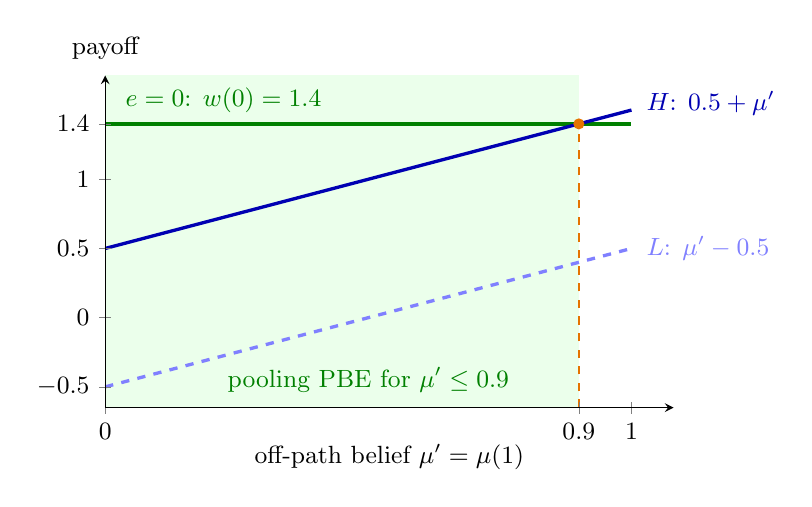
\begin{tikzpicture}[font=\small, >={Latex[length=2mm]}]
  \begin{axis}[
    axis lines=left, xmin=0, xmax=1.08, ymin=-0.65, ymax=1.75,
    xtick={0,0.9,1}, ytick={-0.5,0,0.5,1,1.4},
    xlabel={off-path belief $\mu'=\mu(1)$},
    ylabel={payoff},
    xlabel style={anchor=north, at={(axis description cs:0.5,-0.08)}},
    ylabel style={rotate=-90, anchor=south, at={(axis description cs:0,1.02)}},
    width=8.8cm, height=5.8cm, clip=false, axis on top]
    % beliefs that support pooling
    \fill[green!8] (axis cs:0,-0.65) rectangle (axis cs:0.9,1.75);
    % pooling payoff
    \addplot[green!50!black, very thick, domain=0:1, samples=2] {1.4};
    \node[green!50!black, anchor=south west] at (axis cs:0.02,1.41) {$e=0$: $w(0)=1.4$};
    % deviation payoffs
    \addplot[blue!70!black, very thick, domain=0:1, samples=2] {0.5+x};
    \addplot[blue!50, very thick, dashed, domain=0:1, samples=2] {x-0.5};
    \node[blue!70!black, anchor=west] at (axis cs:1.01,1.55) {$H$: $0.5+\mu'$};
    \node[blue!50, anchor=west] at (axis cs:1.01,0.5) {$L$: $\mu'-0.5$};
    % threshold
    \draw[orange!90!black, thick, dashed] (axis cs:0.9,-0.65) -- (axis cs:0.9,1.4);
    \fill[orange!90!black] (axis cs:0.9,1.4) circle (2pt);
    \node[green!50!black] at (axis cs:0.5,-0.45) {pooling PBE for $\mu'\le0.9$};
  \end{axis}
\end{tikzpicture}
\end{document}
